\documentclass[10pt]{article}
\usepackage[margin=1in]{geometry}
\usepackage[T1]{fontenc}
\usepackage[utf8]{inputenc}
\DeclareUnicodeCharacter{03C4}{\ensuremath{\tau}}
\usepackage{lmodern}
\usepackage{microtype}
\usepackage{booktabs}
\usepackage{graphicx}
\usepackage{xcolor}
\usepackage{amsmath,amssymb}
\usepackage{tikz}
\usetikzlibrary{positioning,arrows.meta}
\usepackage[numbers,sort&compress]{natbib}
\usepackage{hyperref}
\hypersetup{colorlinks=true,linkcolor=blue!50!black,citecolor=blue!50!black,urlcolor=blue!50!black}
\usepackage{listings}
\lstset{basicstyle=\ttfamily\footnotesize,breaklines=true,columns=fullflexible,frame=single}

\newcommand{\fiks}{\textsc{fiks}}
\newcommand{\TODO}[1]{\textcolor{red}{[TODO: #1]}}
% Generated by paper/scripts/pilot_numbers.py from committed logs. Do not edit.
\newcommand{\benchModel}{claude-sonnet-5-5}
\newcommand{\callsB}{47}
\newcommand{\ciHiA}{100.0\%}
\newcommand{\ciHiB}{92.7\%}
\newcommand{\ciHiBd}{75.4\%}
\newcommand{\ciHiBdold}{80.8\%}
\newcommand{\ciHiBold}{60.8\%}
\newcommand{\ciHiC}{100.0\%}
\newcommand{\ciLoA}{88.6\%}
\newcommand{\ciLoB}{66.4\%}
\newcommand{\ciLoBd}{42.3\%}
\newcommand{\ciLoBdold}{48.8\%}
\newcommand{\ciLoBold}{27.4\%}
\newcommand{\ciLoC}{88.6\%}
\newcommand{\costMax}{0.21}
\newcommand{\costMin}{0.11}
\newcommand{\costTotal}{0.77}
\newcommand{\declinedA}{0}
\newcommand{\declinedB}{5}
\newcommand{\declinedBd}{5}
\newcommand{\declinedBdold}{5}
\newcommand{\declinedBold}{15}
\newcommand{\declinedC}{0}
\newcommand{\kTrials}{5}
\newcommand{\minsMax}{1.6}
\newcommand{\minsMin}{1.4}
\newcommand{\nConfirmed}{5}
\newcommand{\nDetected}{5}
\newcommand{\nDrifts}{5}
\newcommand{\nOneAttempt}{5}
\newcommand{\nPrGreen}{5}
\newcommand{\nPrs}{10}
\newcommand{\nPrsClosed}{1}
\newcommand{\nPrsDemoOpen}{4}
\newcommand{\nPrsGreen}{10}
\newcommand{\nPrsMerged}{5}
\newcommand{\nReproValid}{5}
\newcommand{\nTasks}{6}
\newcommand{\nWrongTasksBd}{1}
\newcommand{\noAnswerA}{0}
\newcommand{\noAnswerB}{0}
\newcommand{\noAnswerBd}{2}
\newcommand{\noAnswerBdold}{0}
\newcommand{\noAnswerBold}{2}
\newcommand{\noAnswerC}{0}
\newcommand{\pFiveA}{100.0\%}
\newcommand{\pFiveB}{83.3\%}
\newcommand{\pFiveBd}{50.0\%}
\newcommand{\pFiveBdSens}{66.7\%}
\newcommand{\pFiveBdold}{66.7\%}
\newcommand{\pFiveBold}{33.3\%}
\newcommand{\pFiveC}{100.0\%}
\newcommand{\pOneA}{100.0\%}
\newcommand{\pOneB}{83.3\%}
\newcommand{\pOneBd}{60.0\%}
\newcommand{\pOneBdold}{66.7\%}
\newcommand{\pOneBold}{43.3\%}
\newcommand{\pOneC}{100.0\%}
\newcommand{\pairLosses}{0}
\newcommand{\pairP}{0.50}
\newcommand{\pairWins}{2}
\newcommand{\repairModel}{claude-opus-5-5}
\newcommand{\trialsA}{30}
\newcommand{\trialsB}{30}
\newcommand{\trialsBd}{30}
\newcommand{\trialsBdold}{30}
\newcommand{\trialsBold}{30}
\newcommand{\trialsC}{30}
\newcommand{\turnsMax}{14}
\newcommand{\turnsMedian}{12}
\newcommand{\turnsMin}{10}
\newcommand{\vOneCalls}{37}
\newcommand{\vOneFpUpper}{9.4\%}
\newcommand{\vOneTrialFpUpper}{11.4\%}
\newcommand{\vOneViolated}{0}
\newcommand{\violatedCallsB}{41}
\newcommand{\wrongA}{0}
\newcommand{\wrongB}{0}
\newcommand{\wrongBd}{5}
\newcommand{\wrongBdold}{5}
\newcommand{\wrongBold}{0}
\newcommand{\wrongC}{0}
\newcommand{\wrongTasksBd}{T5}


\title{\fiks: Turning Silent Tool Failures into Gated Repair Pull Requests\\for MCP Servers\\[4pt]
\large System Design, Pilot Evaluation, and a Pre-Registration Draft}
\author{\TODO{author names and affiliations}\\\small Repository owner: \texttt{github.com/vats98754}}
\date{Preprint, October 2026}

\begin{document}
\maketitle

\begin{abstract}
Agents are meant to obtain ``ground truth'' from tool results at each step~\cite{anthropic2024agents}, yet MCP servers can return well-formed \emph{successful} responses despite incorrect behaviour~\cite{owotogbe2026mcpfaults}, and agents given empty or malformed success payloads often fabricate results~\cite{singh2026scapegoats}.
Runtime monitors can warn the current agent~\cite{panthi2026outcomemonitors}, but the tool stays broken for every later agent, and spec-diff tools are blind when an upstream API changes behaviour without changing its schema~\cite{oasdiff-breaking}.
We present \fiks, which closes this loop for MCP servers.
A proxy checks every successful tool result against an \emph{outcome contract} (ranges, nullness, counts, freshness, agreement with the raw upstream HTTP exchange, read-after-write), and returns a receipt to the agent.
On a violation it captures the exact call and upstream exchange, compiles it into a deterministic reproduction test that must fail on the current code \emph{for the named property}, and asks a coding agent to repair the server.
\fiks{} opens a pull request only after that test, the full contract suite, every stored trace, typecheck, lint and CI on the exact commit all pass, and it never merges.
In a pilot on one mock vendor with \nDrifts{} seeded behavioural drifts whose OpenAPI document is unchanged, \fiks{} flagged all \nDetected{} drifts, produced a valid fail-first repro for each, and obtained a green-CI pull request in one repair attempt per drift (\minsMin--\minsMax{} minutes from captured violation to PR; \$\costMin--\$\costMax{} API-price estimate per repair).
In a \nTasks-task, \kTrials-trial agent bench, pass$^5$ was \pFiveBd{} without \fiks{}, \pFiveB{} with receipts and \pFiveC{} after the fixes were merged; with only \pairWins{} discordant tasks the receipts-vs-no-\fiks{} difference is not statistically significant (two-sided sign test $p=\pairP$), and an earlier receipt wording performed \emph{worse} than no monitor (\pFiveBold{} vs \pFiveBdold; \pairLossesOld{} tasks worse, \pairWinsOld{} better, $p=\pairPOld$).
From a catalog of 508 sources (505 verified or metadata-corrected, 3 unreachable) we argue that the defensible novelty is the combination of trigger, artifact and gate placement, not any component.
We release a pre-registration draft for a confirmatory study (four hypotheses, Holm-corrected); it has not yet been frozen or registered, and none of its experiments have been run.
\end{abstract}

\section{Introduction}
\label{sec:intro}

Agents act on what tools tell them.
Anthropic describes agents as systems that must obtain ``ground truth'' from the environment, such as tool results, at each step~\cite{anthropic2024agents}; in the Model Context Protocol (MCP) that ground truth arrives as tool results.
When a tool fails loudly, with an exception or an error result, existing machinery handles it: the agent retries, the error tracker files an issue, and coding agents can be pointed at the stack trace~\cite{sentry-seer-issue-fix,devin-oncall}.
The harder case is a tool that fails \emph{silently}.
A study of 833 MCP runtime-fault threads found servers that return well-formed success responses despite incorrect behaviour~\cite{owotogbe2026mcpfaults}.
Agents given HTTP 200 responses with empty, null or malformed payloads fabricated results in 56.6\% of valid responses~\cite{singh2026scapegoats}; on $\tau^2$-bench no LLM-judge configuration exceeded AUROC 0.65 at detecting false success~\cite{advani2026falsesuccess}; and even the tools inside agent benchmarks report writes that never happened~\cite{bellibatlu2026contractaudit}.

A common source of silent failure is upstream drift: the vendor API behind an MCP server changes behaviour (a unit, a field name, pagination, a timestamp format, a write that now needs a header) while its published schema stays the same.
Spec-diff tools compare documents and therefore report nothing~\cite{oasdiff-breaking}; in npm, about two thirds of documented breaking changes are behavioural rather than signature changes~\cite{kong2025npm}.
Runtime outcome monitors close part of the gap: they check results and tell the running agent~\cite{panthi2026outcomemonitors,verimcp}.
But detection alone leaves the tool broken for every later session, model and user.

\fiks{} turns the runtime violation into a durable fix.
Its premise is that a violation observed in live traffic is already most of a reproduction: the exact arguments, the raw upstream exchange and the property that failed.
Work on test-driven repair identifies writing a valid reproduction test as the bottleneck~\cite{tdflow} and finds such tests hard to generate~\cite{mundler2024swtbench,otter}; it also warns that fail-to-pass tests can still be lax~\cite{tan2026coharden} or admit partial patches~\cite{swe-doctor}.
\fiks{} therefore (i)~compiles the trace into a test that must fail on the current code \emph{for the stated reason}, (ii)~gives that test to a tool-restricted coding agent, and (iii)~places every gate, including CI on the exact commit, \emph{before} a pull request is opened.

\paragraph{Contributions.}
\begin{enumerate}
  \item \textbf{A loop and its gate placement} (\S\ref{sec:design}): per-call outcome contracts on successful MCP results, an immediate receipt to the agent, trace capture with the raw upstream exchange, a named-property fail-first reproduction, gated repair, and a pull request that is never merged automatically.
  \item \textbf{An implementation and a pilot evaluation} (\S\ref{sec:pilot}) on five seeded drifts, with every number produced by a script from committed logs (Tables~\ref{tab:loop}--\ref{tab:receipts}), including a negative result on receipt wording.
  \item \textbf{A positioning against a catalog of 508 sources} (\S\ref{sec:related}), with an explicit list of what is \emph{not} new.
  \item \textbf{A pre-registration draft} (\S\ref{sec:protocol}) with design, power analysis and analysis plan, to be frozen (tag \texttt{prereg-v1}) before any confirmatory run.
\end{enumerate}

\paragraph{Scope.} This paper reports a pilot. Its evidence comes from one mock vendor, one MCP server, drifts and contracts written by the same authors, six agent tasks and one model family. We say in \S\ref{sec:limits} what the pilot cannot show, and the protocol in \S\ref{sec:protocol} is designed to test it.

\section{Problem: silent failures at the agent--tool boundary}
\label{sec:problem}

Let a tool $\tau$ map arguments $x$ to a result $r=\tau(x)$ by calling an upstream service $U$; the call produces an upstream exchange $e=(\mathrm{req},\mathrm{resp})$.
A \emph{silent failure} is a call where $r$ is a well-formed success (no exception, no \texttt{isError}, valid against the declared \texttt{outputSchema}) but $r$ misstates the state of $U$.
The MCP specification lets a tool declare an \texttt{outputSchema} for its structured content, with output validation left to clients~\cite{mcp-spec-2026-07-28-tools}; a schema can check shape, not whether a price is in dollars or cents.

We focus on \emph{upstream behavioural drift}: $U$ changes at time $t_0$ while its published specification and $\tau$'s code do not.
From $t_0$ on, every call that touches the changed behaviour is silently wrong, for every agent, until $\tau$ is fixed.
Three properties make this setting tractable for a closed loop:
(a)~the violation is observable per call, because the proxy sees both $r$ and $e$;
(b)~the trace $(x, e, r, \text{property})$ is a deterministic reproduction once $e$ is replayed;
(c)~the fix belongs to $\tau$'s repository, so it can be proposed as a pull request and reviewed.

\section{Design of \fiks}
\label{sec:design}

\begin{figure}[t]
\centering
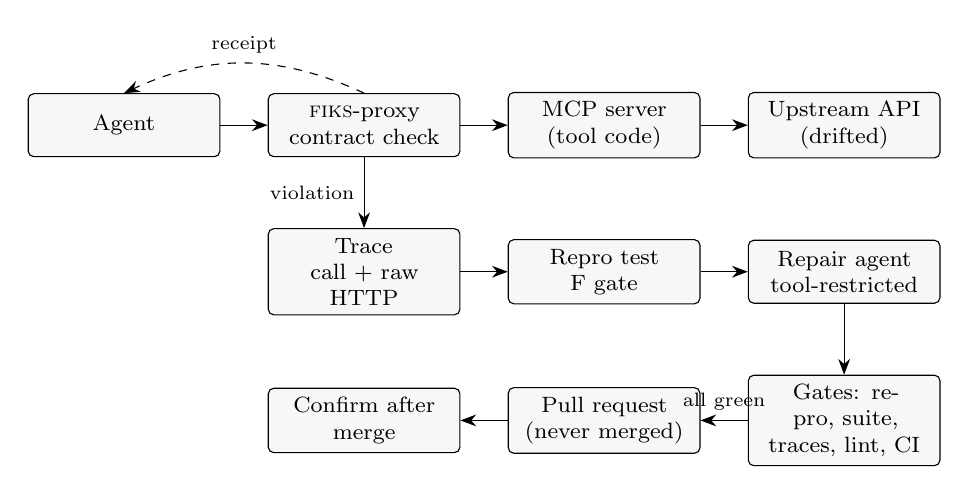
\begin{tikzpicture}[node distance=4mm and 6mm, every node/.style={font=\footnotesize},
  box/.style={draw, rounded corners=2pt, align=center, minimum height=8mm, text width=22mm, fill=gray!6},
  arr/.style={-{Stealth[length=2mm]}}]
\node[box] (agent) {Agent};
\node[box, right=of agent] (proxy) {\fiks-proxy\\contract check};
\node[box, right=of proxy] (server) {MCP server\\(tool code)};
\node[box, right=of server] (vendor) {Upstream API\\(drifted)};
\node[box, below=9mm of proxy] (trace) {Trace\\call + raw HTTP};
\node[box, right=of trace] (repro) {Repro test\\F gate};
\node[box, right=of repro] (repair) {Repair agent\\tool-restricted};
\node[box, below=9mm of repair] (gates) {Gates: repro, suite,\\traces, lint, CI};
\node[box, left=of gates] (pr) {Pull request\\(never merged)};
\node[box, left=of pr] (confirm) {Confirm after\\merge};
\draw[arr] (agent) -- (proxy); \draw[arr] (proxy) -- (server); \draw[arr] (server) -- (vendor);
\draw[arr, dashed] (proxy.north) to[bend right=25] node[above, font=\scriptsize]{receipt} (agent.north);
\draw[arr] (proxy) -- node[left, font=\scriptsize]{violation} (trace);
\draw[arr] (trace) -- (repro); \draw[arr] (repro) -- (repair); \draw[arr] (repair) -- (gates);
\draw[arr] (gates) -- node[above, font=\scriptsize]{all green} (pr); \draw[arr] (pr) -- (confirm);
\end{tikzpicture}
\caption{The \fiks{} loop. The receipt reaches the running agent immediately; the fix reaches every later agent once the pull request is merged (\fiks{} never merges).}
\label{fig:loop}
\end{figure}

\subsection{Outcome contracts and receipts}
A contract is a per-tool list of invariants evaluated on each successful result (Table~\ref{tab:vocab}).
Most kinds resemble schema and anomaly checks in data validation systems~\cite{tfdv-2019}; two kinds use the proxy's position between tool and upstream.
\texttt{equalsUpstream} compares a result field with the field the upstream actually sent in the same call, and \texttt{readAfterWrite} re-reads a created resource from the upstream to confirm a write persisted.
Each verdict is \emph{verified}, \emph{violated} or \emph{unverifiable}.
The proxy attaches a receipt to the result in three places: MCP \texttt{\_meta}, a final text block, and a field in \texttt{structuredContent}, because some clients show the model only the structured content.
A receipt states the violated property, the upstream facts the proxy observed, and what the agent should not do with the value. The receipt for the pilot's renamed-price drift reads:
\begin{lstlisting}
[fiks] VIOLATED get_product: price is null, but p-1001 should have one; vendor sent unit_amount = 1199 (in 20-2000 USD). Don't say there is no price; if you use the vendor value, say unconfirmed.
\end{lstlisting}

\begin{table}[t]
\centering\small
\caption{Contract vocabulary used in the pilot. The first five kinds are standard data-quality checks; the last two rely on seeing the upstream exchange of the same call.}
\label{tab:vocab}
\begin{tabular}{ll}
\toprule
Kind & Checks \\
\midrule
\texttt{range} & numeric field within $[\min,\max]$ in a stated unit \\
\texttt{notNull}, \texttt{nonEmpty} & field present / list non-empty for known-good inputs \\
\texttt{unique} & no duplicate ids in a list \\
\texttt{countMatchesTotal} & returned items equal the reported total \\
\texttt{freshness} & timestamp within a plausible window of the call time \\
\texttt{equalsUpstream} & field equals the upstream response's field (JSON or instant) \\
\texttt{readAfterWrite} & a created resource can be read back from the upstream \\
\bottomrule
\end{tabular}
\end{table}

\subsection{Trace, reproduction and the F gate}
On a violation the proxy stores a trace: tool, arguments, the raw upstream requests and responses recorded by an HTTP tap, the contract and the violated property ids.
\fiks{} generates a test in the server's own repository that replays the recorded upstream exchange through the server's real code and asserts the contract.
The \textbf{F gate} accepts the test only if it fails on the current code on every one of several runs (three in the current code; two in the earliest pilot runs, Table~\ref{tab:loop}), and the first failure line names exactly the target property ids; a test that fails for another reason, or passes, is rejected.
This makes ``fails for the stated reason'' a deterministic check that needs no reference patch, unlike fail-to-pass validation against a gold patch~\cite{mundler2024swtbench} or heuristic checks on the failure~\cite{otter}.

\subsection{Repair and gates}
A coding agent (Claude Agent SDK; \repairModel{} in the pilot) receives the violation, the trace and the failing test in an isolated git worktree.
A tool-permission callback lets it write only under \texttt{src/}, run only the project's typecheck, lint and test commands, and read only inside the worktree; tests, fixtures and traces are hashed at the snapshot, and any change to them fails the run.
When a correct fix changes upstream requests (for example, a new required header), \fiks{} itself re-records the affected fixtures from the committed recordings with a frozen clock, in a separate commit containing only re-recordings.
The \textbf{P gate} then requires the repro to pass, together with the full contract suite, every stored trace, typecheck and lint.
\fiks{} pushes the branch, waits for CI on that exact commit, and opens a pull request only if CI is green; if the pull request's head differs from the commit that passed CI, it is closed.
The pull request body states what broke, the trace, the test, the diff, before/after results and the gate outcomes, and says that a green suite is not a proof of correctness.
\fiks{} never merges. After a merge, \texttt{fiks confirm} re-runs each repaired call live and replays every stored trace.

\section{Pilot evaluation}
\label{sec:pilot}

\subsection{Setup}
\paragraph{Substrate.} A mock vendor API with a version switch (v1, v2) and an MCP server (\texttt{shop-mcp}, four tools: \texttt{search\_products}, \texttt{get\_product}, \texttt{create\_order}, \texttt{get\_order}) in its own repository, so pull requests and CI are real. The vendor's OpenAPI document is identical in v1 and v2. Version v2 introduces \nDrifts{} drifts (Table~\ref{tab:drifts}). We wrote the drifts and the contracts; \S\ref{sec:limits} discusses the circularity this creates.

\begin{table}[t]
\centering\small
\caption{Seeded behavioural drifts (vendor v2). The OpenAPI document does not change.}
\label{tab:drifts}
\begin{tabular}{lll}
\toprule
Drift & Upstream change & Silent symptom in the unfixed tool \\
\midrule
D1 unit & prices become integer cents, same field name & prices 100$\times$ too high \\
D2 rename & \texttt{price} renamed to \texttt{unit\_amount} & price returned as \texttt{null} \\
D3 lost write & order persists only with a new required header & create succeeds; order cannot be read back \\
D4 pagination & search results paginated & only page 1 returned; count $<$ total \\
D5 timestamp & ISO-8601 becomes epoch milliseconds & dates parsed as 1970 \\
\bottomrule
\end{tabular}
\end{table}

\paragraph{Agent bench.} \nTasks{} tasks (T1--T5 each exposed to one drift; T6 a control), \kTrials{} trials each, agent \benchModel{} via the Claude Agent SDK with only the shop MCP server and a \texttt{submit\_answer} tool. A deterministic grader compares the submitted answer with the vendor's ground truth; a hedged wrong value counts as wrong, and an answer never submitted counts as a failure (reported separately as ``no answer''). Phases: before drift through \fiks; after drift without \fiks{} (agent talks to the server directly); after drift with \fiks{} receipts; after drift with the \nPrsMerged{} \fiks{} pull requests merged. pass$^k$ uses the unbiased $\binom{c}{k}/\binom{n}{k}$ estimator averaged over tasks~\cite{yao2024taubench,chen2021codex}; intervals are Wilson~\cite{brown2001binomial}, computed over trials and therefore ignoring clustering by task, which can make them too narrow~\cite{bowyer2025clt}.

\paragraph{Provenance.} All numbers in this section are emitted by \texttt{paper/scripts/pilot\_numbers.py} from committed logs (\texttt{bench/results/}, repair records, and a snapshot of the pull requests); \texttt{--check} rebuilds them and fails on any difference. Phases A, B and B-direct used \fiks{} commit \texttt{\fiksSha} and the server at tag \texttt{seed-v1} (\texttt{\shopShaAB}); phase C used the server's main branch at \texttt{\shopShaC} (the \nPrsMerged{} fix pull requests plus a test-harness pull request). \nDirtyRuns{} of these four runs record a dirty \fiks{} tree; at the time this flag also counted untracked bench output folders. The receipt-v1 runs and the D1--D3, D5 repairs (2026-10-18) ran from an uncommitted tree that predates commit \texttt{8c7daa8}; the D4 repair ran from an uncommitted tree before \texttt{\fiksSha}.

\subsection{Detection and false alarms}
In the drift phase, \violatedCallsB{} of \callsB{} tool calls received a violated receipt, covering the violated properties of all five drifts (D1 \texttt{items.price.range}, D2 \texttt{price.notNull}, D3 \texttt{readAfterWrite}, D4 \texttt{countMatchesTotal}, D5 \texttt{created\_at} freshness and upstream agreement).
On clean v1 traffic, \vOneViolated{} of \vOneCalls{} calls were flagged (Wilson 95\% upper bound \vOneFpUpper{} per call; \vOneTrialFpUpper{} per trial over \trialsA{} trials).
These bounds are weak: the pilot's clean traffic is small and comes from the same six tasks the contracts were written against.

\subsection{The repair loop}
Table~\ref{tab:loop} reports the loop for each drift. Each loop was triggered by a fixed one-call scenario against vendor v2, not by the bench agent's calls.
All \nReproValid{} reproductions passed the F gate with the named property ids (\nFThreeRuns{} on three runs; \nFTwoRuns{}, run on 2026-10-18, on two runs, the setting used then), all \nOneAttempt{} repairs succeeded in one agent attempt (\turnsMin--\turnsMax{} turns, median \turnsMedian), and all \nPrGreen{} pull requests had green CI before opening.
Total repair cost was \$\costTotal{} at API list prices; the runs used a subscription token, so this is an estimate, not a bill.
After the \nPrsMerged{} pull requests (and the harness pull request) were merged by an AI coding assistant on the owner's account at the owner's request, without line-by-line review, \texttt{fiks confirm} found each drift resolved (\nConfirmed/\nDrifts).
Across the pilot and later demonstration runs, \fiks{} opened \nPrs{} repair pull requests, all with green checks; \nPrsMerged{} were merged, \nPrsDemoOpen{} demonstration pull requests target throw-away branches and remain open, and \nPrsClosed{} was a duplicate opened by an operator error and closed.
These merges are not evidence of maintainer acceptance, which large-scale studies of agent pull requests measure separately~\cite{ehsani2026failedagenticprs}.

\begin{table}[t]
\centering\small
\caption{Repair loop per drift. ``Min.\ to PR'' runs from the captured violation to the opened pull request, including the CI wait. Cost is the Agent SDK's API-price estimate.}
\label{tab:loop}
\resizebox{\linewidth}{!}{% Generated by paper/scripts/pilot_numbers.py. Do not edit.
\begin{tabular}{llcrrrrlcc}
\toprule
Drift & Violated property & F gate & Att. & Turns & Cost (\$) & Min. to PR & PR & Merged & Confirmed \\
\midrule
D1 & \texttt{items.price.range} & yes & 1 & 13 & 0.11 & 1.4 & \#2 & yes & yes \\
D2 & \texttt{price.notNull} & yes & 1 & 10 & 0.14 & 1.4 & \#1 & yes & yes \\
D3 & \texttt{readAfterWrite} & yes & 1 & 14 & 0.21 & 1.6 & \#3 & yes & yes \\
D4 & \texttt{countMatchesTotal} & yes & 1 & 11 & 0.19 & 1.5 & \#7 & yes & yes \\
D5 & \texttt{created\_at.freshness, created\_at.equalsUpstream} & yes & 1 & 12 & 0.12 & 1.4 & \#4 & yes & yes \\
\bottomrule
\end{tabular}
}
\end{table}

\subsection{Agent outcomes}
Table~\ref{tab:bench} gives pass$^k$ per phase and Table~\ref{tab:tasks} the per-task successes.
Without \fiks, pass$^5$ fell from \pFiveA{} to \pFiveBd{}; with receipts it was \pFiveB; with the fixes merged it returned to \pFiveC{} with no receipts needed.
Three observations temper this.
First, only \pairWins{} tasks differ in the receipts-vs-no-\fiks{} comparison (\pairLosses{} in the other direction), so a task-level paired sign test gives $p=\pairP$; the pilot cannot establish an effect.
Second, all \wrongBd{} wrong answers without \fiks{} came from one task (\wrongTasksBd, the timestamp drift: the agent reported 1970), and \noAnswerBd{} further failures were trials where the agent stated the correct price but never submitted it; counting those as correct would raise the no-\fiks{} pass$^5$ to \pFiveBdSens{}, about half the gap.
Third, the \declinedB{} declines with receipts are all the lost-write task T3, where the vendor really did not persist the order; ``could not confirm'' is arguably the right answer there, the grader counts it as a failure, and the same \declinedBd{} declines occur without \fiks.

\begin{table}[t]
\centering\small
\caption{Agent bench (\benchModel, \nTasks{} tasks $\times$ \kTrials{} trials per phase). pass$^1$ CI is Wilson over trials and ignores clustering by task.}
\label{tab:bench}
\resizebox{\linewidth}{!}{% Generated by paper/scripts/pilot_numbers.py. Do not edit.
\begin{tabular}{lrrrrrcrrrrr}
\toprule
Phase & \multicolumn{5}{c}{pass$^k$ (\%), $k{=}1..5$} & pass$^1$ 95\% CI & Corr. & Wrong & Decl. & No ans. & Viol. calls \\
\midrule
Before drift (v1), through fiks & 100.0 & 100.0 & 100.0 & 100.0 & 100.0 & 89--100 & 30 & 0 & 0 & 0 & 0 \\
After drift (v2), no fiks & 60.0 & 55.0 & 51.7 & 50.0 & 50.0 & 42--75 & 18 & 5 & 5 & 2 & 0 \\
After drift (v2), fiks receipts & 83.3 & 83.3 & 83.3 & 83.3 & 83.3 & 66--93 & 25 & 0 & 5 & 0 & 41 \\
After drift (v2), fiks fixes merged & 100.0 & 100.0 & 100.0 & 100.0 & 100.0 & 89--100 & 30 & 0 & 0 & 0 & 0 \\
\bottomrule
\end{tabular}
}
\end{table}

\begin{table}[t]
\centering\small
\caption{Per-task successes out of \kTrials. T1--T5 are each exposed to one drift (D2, D1, D3, D4, D5); T6 is a control.}
\label{tab:tasks}
% Generated by paper/scripts/pilot_numbers.py. Do not edit.
\begin{tabular}{lcccccc}
\toprule
Phase & T1 & T2 & T3 & T4 & T5 & T6 \\
\midrule
Before drift (v1), through fiks & 5/5 & 5/5 & 5/5 & 5/5 & 5/5 & 5/5 \\
After drift (v2), no fiks & 3/5 & 5/5 & 0/5 & 5/5 & 0/5 & 5/5 \\
After drift (v2), fiks receipts & 5/5 & 5/5 & 0/5 & 5/5 & 5/5 & 5/5 \\
After drift (v2), fiks fixes merged & 5/5 & 5/5 & 5/5 & 5/5 & 5/5 & 5/5 \\
\bottomrule
\end{tabular}

\end{table}

\subsection{A negative result: receipt wording}
Receipts are part of the method. Our first wording (v1) stated the violation and told the agent not to quote the flagged value; apart from the timestamp drift, whose receipt is unchanged in v2, it neither gave the upstream value the tool had dropped nor suggested a next step other than telling the user the value was unavailable or unconfirmed.
With it, pass$^5$ was \pFiveBold{} against \pFiveBdold{} without \fiks{} on the same day (Table~\ref{tab:receipts}; \pairLossesOld{} tasks worse, \pairWinsOld{} better, sign test $p=\pairPOld$): the agent declined \declinedBold{} times (all trials of T1, T2 and T3; the T3 declines also occur without \fiks) and \noAnswerBold{} times gave no answer.
The second wording (v2) adds the upstream value the tool dropped, labelled unconfirmed, and next steps. We changed the wording after seeing these results, so the v2 numbers are post hoc and need the independent test in \S\ref{sec:protocol}.

\begin{table}[t]
\centering\small
\caption{Receipt wording history on the drifted vendor (same tasks and model). v1 lowered success below no monitor.}
\label{tab:receipts}
% Generated by paper/scripts/pilot_numbers.py. Do not edit.
\begin{tabular}{lrrrrr}
\toprule
Arm (drifted vendor) & pass$^1$ & pass$^5$ & Wrong & Declined & No answer \\
\midrule
No fiks (2026-10-18 run) & 66.7 & 66.7 & 5 & 5 & 0 \\
fiks receipts, wording v1 & 43.3 & 33.3 & 0 & 15 & 2 \\
No fiks (2026-10-20 run) & 60.0 & 50.0 & 5 & 5 & 2 \\
fiks receipts, wording v2 & 83.3 & 83.3 & 0 & 5 & 0 \\
\bottomrule
\end{tabular}

\end{table}

\section{Related work and novelty boundary}
\label{sec:related}

\paragraph{Silent failures and agent benchmarks.} MCP fault studies classify silent faults from issue threads but do not reproduce or repair them~\cite{owotogbe2026mcpfaults}. Controlled injection of silent failures into tool stubs shows agents fabricating results~\cite{singh2026scapegoats}, and false success is hard to detect from transcripts~\cite{advani2026falsesuccess}. Benchmarks that grade tool-using agents assume tools do what they advertise; an executable-contract audit found seven tool defects, including success messages for writes that never happened~\cite{bellibatlu2026contractaudit}. $\tau$-bench's tools are deterministic functions over JSON databases~\cite{yao2024taubench}.

\paragraph{Runtime monitors.} Outcome Monitors check results and give the agent recovery affordances, explicitly without repairing the tool~\cite{panthi2026outcomemonitors}; verimcp re-derives outcomes after git, file and CI calls~\cite{verimcp}; a tool wrapper combining postcondition verification, verify-before-retry and idempotency keys reduced duplicate actions in simulation~\cite{mansoor2026verifiedtoolcalls}. Action-side enforcement such as AgentSpec checks planned actions rather than results~\cite{agentspec}. \fiks{}'s receipt step belongs to this line and is not new on its own.

\paragraph{Specification, contract and data validation.} Spec-diff tools find nothing when the document does not change~\cite{oasdiff-breaking}; consumer-driven contracts need the provider to run consumer pacts~\cite{pact-how-it-works}; schema-derived fuzzing finds schema violations~\cite{hatfielddodds2022schemathesis}. Large-scale studies count breaking changes in library APIs~\cite{xavier2017apibreak,kong2025npm}. Data validation systems enforce similar presence, range and distribution checks on batches~\cite{tfdv-2019}, and invariant inference goes back to Daikon~\cite{daikon}. Record/replay tools turn captured traffic into regression tests whose oracle is the old response~\cite{keploy}; that oracle encodes the bug when the recording is made after the drift.

\paragraph{Reproduction and repair.} Issue-to-test generation is hard and its validity is judged by fail-to-pass execution~\cite{libro,mundler2024swtbench,otter}; a true reproduction is the bottleneck of test-driven repair~\cite{tdflow}, yet fail-to-pass tests can be lax~\cite{tan2026coharden} or admit partial patches~\cite{swe-doctor}, and in a self-healing agent harness 55\% of gate-rejected instruction changes improved their trigger while regressing a protected case~\cite{tayebati2026selfhealingharness}. Repair systems start from issues~\cite{swe-agent,agentless}, compile errors after a dependency bump~\cite{reyes2025byam}, or an upstream breaking change with no localizing failing test~\cite{yang2026deprepair}. Structured upstream evidence helps dependency repair while raw evidence hurts~\cite{yang2026deprepair}, which motivates compiling the trace into a test rather than pasting it.

\paragraph{Production-driven and commercial loops.} ClearView patched deployed software from learned invariants~\cite{perkins2009clearview}; Itzal validated production-driven patches on traffic~\cite{durieux2016itzal}; SapFix shipped detect--test--repair with human approval~\cite{marginean2019sapfix}. In 2026, observability and alerting products open fix pull requests from errors, incidents or LLM scans and iterate CI after opening~\cite{sentry-seer-issue-fix,posthog-anatomy-pr,devin-oncall,langsmith-changelog-2026}, and some measure recurrence after fixes~\cite{cleric-verifying-fixes}. AegisFlow detects silent pipeline drift statistically and deploys validated patches autonomously for pre-approved failure classes~\cite{awan2026aegisflow}. A granted patent claims language-model repair of a detected issue from its error information, with dependent claims adding a pull request accompanied by a software test~\cite{msft-us12711009}.

\paragraph{What is and is not new.} Table~\ref{tab:matrix} compares the closest systems by loop step, from their documentation or papers. Each step exists somewhere. In the sources we reviewed (searched up to 2026-10-21; patent databases only partly searched), we found no system that combines: a trigger that is a deterministic contract violation in a \emph{successful} tool result, checked per call against the raw upstream exchange; a committed test that must fail first for the named property; and all gates, including CI on the exact commit, before the pull request opens, with a receipt to the agent while the fix is pending. We claim only that combination, and the pilot does not yet show that it outperforms a composition of existing parts; that is the question of \S\ref{sec:protocol}.

\begin{table}[t]
\centering\scriptsize
\caption{Loop steps covered by the closest systems (Y documented; P partial or different form; N not done or not described, and absence from documentation is not proof; ? documentation silent on the step). Sem: semantic check of a successful result; Rcpt: verdict to the agent; Trace: raw upstream captured; F: test must fail first for the stated reason; Gates: suite and CI pass before the PR.}
\label{tab:matrix}
\begin{tabular}{lccccccccc}
\toprule
System & Sem & Rcpt & Trace & Repro test & F & Fix & Gates & PR & Confirm \\
\midrule
\fiks{} (this paper) & Y & Y & Y & Y & Y & Y & Y & Y & Y \\
Outcome Monitors~\cite{panthi2026outcomemonitors} & Y & Y & N & N & N & N & N & N & N \\
verimcp~\cite{verimcp} & Y & Y & P & N & N & N & N & N & N \\
AegisFlow~\cite{awan2026aegisflow} & Y & N & P & N & N & Y & P & N & Y \\
LangSmith Engine~\cite{langsmith-changelog-2026} & P & N & P & N & P & Y & N & Y & Y \\
Cleric~\cite{cleric-verifying-fixes} & P & N & P & N & N & Y & ? & Y & Y \\
PostHog Self-driving~\cite{posthog-anatomy-pr} & N & N & P & Y & ? & Y & N & Y & ? \\
Sentry Seer~\cite{sentry-seer-issue-fix} & N & N & P & P & N & Y & N & Y & N \\
Keploy~\cite{keploy} & N & N & Y & Y & N & N & N & N & N \\
SapFix~\cite{marginean2019sapfix} & N & N & P & Y & P & Y & P & Y & N \\
Itzal~\cite{durieux2016itzal} & P & N & P & N & P & Y & P & P & N \\
\bottomrule
\end{tabular}
\end{table}

\section{Confirmatory protocol (pre-registration draft)}
\label{sec:protocol}

The draft pre-registration is \texttt{paper/prereg/PREREG.md}, sourced from \texttt{paper/PLAN.md}; it becomes binding only when tagged \texttt{prereg-v1}, and amendments made before that are logged in \texttt{PLAN.md} \S0.B. It was produced by competing designs, a judge panel and repeated adversarial critique, and its power numbers are recomputed by script. No confirmatory run has been performed, and part of the required tooling is still being built. The protocol compares \fiks{} with two strong alternatives built on the same monitor, model, budget and sandbox: \textbf{L1}, the same agent and gates with a pre-PR replay of the triggering trace but no visible reproduction test; and \textbf{COMP}, the strongest documented composition, monitor $\rightarrow$ alert $\rightarrow$ coding agent $\rightarrow$ PR $\rightarrow$ CI with source-run replay. Four hypotheses form the confirmatory family (Holm, FWER 0.05):
\begin{description}
  \item[H1 (trigger).] On a frame (fixed in the draft) of at least 1{,}500 blind-authored catalog entities over two domains, fewer than 2\% of entities give rise to any false positive (exact binomial test), with fewer than 1\% of inputs flagged.
  \item[H2 (artifact).] Over a fixed, arm-independent patch pool graded by a held-out oracle, the trace-derived named-property repro has higher balanced accuracy than a fail-first repro written by a coding agent from the same alert, raw trace and replay helper.
  \item[H3 (visible repro).] \fiks{} exposes fewer green-but-incorrect pull requests than L1, with a correct-PR loss no larger than 0.10 (intersection--union test with a direction guard).
  \item[H4 (vs composition).] The same comparison against COMP.
\end{description}
Drifts are authored blind to the contracts by a separate process and applied by a third-party response-rewriting injector; benign upstream evolution, mutation operators frozen before contracts, four real silent-failure bugs in public MCP servers, to be reproduced in private clones, and an adversarial-trace security suite are exploratory arms. Expected losses are stated in the draft as well: out-of-vocabulary string corruption, legitimate evolution that a fixed contract misreads as a fault, and cases where issue text already explains the bug.

\section{Threats to validity and limitations}
\label{sec:limits}

\paragraph{Circularity.} The same authors wrote the drifts, the contracts and the tasks; detection of D1--D5 is therefore close to a construction property. Mutation-based oracle assessment and real faults are needed to measure what contracts miss~\cite{jahangirova2016oracle,just2014mutants}, and runtime contract vocabularies have known blind spots on out-of-vocabulary faults~\cite{panthi2026outcomemonitors}.
\paragraph{Scale and statistics.} \nTasks{} tasks and \kTrials{} trials cannot support task-level significance; trial-level intervals ignore clustering~\cite{bowyer2025clt}. The false-alarm bound comes from \vOneCalls{} clean calls.
\paragraph{Partial or overfitted patches.} A green suite shows the repro and the recorded contracts pass; it does not prove correctness~\cite{swe-doctor,tan2026coharden}. The pilot measured no held-out oracle.
\paragraph{Security.} The repair agent reads attacker-controllable vendor bytes and its code runs in tests. Restricting terminal access does not stop injected agents from writing malicious source~\cite{liu2025aishelljack}, test-passing patches can hide vulnerabilities~\cite{chen2025swexploit}, and injection through tool output is measurable~\cite{debenedetti2024agentdojo,bouras2026capscope}. In the pilot the agent ran without an OS or network sandbox; a container backend and an injection suite are part of the protocol, not of these results.
\paragraph{Legitimate evolution.} A fixed contract cannot tell a vendor fault from an intended change; the pilot always proposed a code fix. A contract-update outcome is designed but unevaluated.
\paragraph{Pilot build differences.} \nFTwoRuns{} of \nDrifts{} F gates ran twice rather than three times; all five repairs and the receipt-v1 runs used uncommitted code; and every repair was triggered by a scripted call, not by agent traffic.
\paragraph{External validity.} One mock vendor, one server, one model family (Claude) for both bench and repair, and seeded rather than organic drift. Merged pull requests were merged by an AI assistant at the owner's request without line-by-line review, so they say nothing about maintainer acceptance.

\section{AI use and ethics statement}
The system, the experiments and this manuscript were produced with substantial assistance from Claude (Claude Code and the Claude Agent SDK; claude-opus-5-5 and claude-sonnet-5-5), directed by the authors. Literature search and source verification were done by agents that recorded the supporting passage for each citation; every number in \S\ref{sec:pilot} is generated from committed logs by a script. The authors are responsible for all claims. No third-party repository was written to: pull requests were opened only on repositories owned by the authors, and real-bug reproductions use private clones.

\section{Conclusion}
\fiks{} shows that a silent tool failure caught by the proxy on a call against a drifted vendor can be turned, within minutes, into a named-property failing test and a gate-passing pull request against the tool. The pilot demonstrates feasibility on seeded drifts; it does not show that the loop beats a composition of existing monitors and coding agents, that its contracts generalize beyond the drifts they were written for, or that its pull requests would be accepted. The draft protocol is designed to answer exactly those questions.

\bibliographystyle{plainnat}
\bibliography{references}

\appendix
\section{Reproducing the pilot numbers}
\begin{lstlisting}
python3 paper/scripts/pilot_numbers.py --check   # rebuild every macro and table from bench/results
python3 paper/scripts/make_bib.py --check        # references.bib from verified sources only
pnpm fiks summarize --check                      # bench summary.json matches the trial logs
pnpm fiks vendor-diff                            # OpenAPI identical across v1/v2; five behaviours differ
pnpm demo --drifts D2 --base fresh               # one live loop: violation -> repro -> repair -> green CI -> PR
\end{lstlisting}
{\sloppy Bench runs: \texttt{bench/results/\{A\_v1,B\_v2,B\_v2\_direct,C\_v2\_fixed\}\_20261020T*}; receipt-v1 history: \texttt{*\_20261018T*}. Repair records: \texttt{bench/results/loop/repairs/}. Pull-request snapshot: \texttt{paper/results/pilot/prs.json}.\par}

\section{Bench tasks}
\begin{tabular}{lll}
\toprule
Task & Drift & Prompt (abridged) \\
\midrule
T1 & D2 & price in US dollars of product p-1001 \\
T2 & D1 & which laptop costs less than \$800 \\
T3 & D3 & buy 2 units of p-1004 and make sure the order exists \\
T4 & D4 & how many products in the ``cable'' category \\
T5 & D5 & on what date was order o-5001 placed \\
T6 & -- & name of product p-1101 (control) \\
\bottomrule
\end{tabular}

\end{document}
